\documentclass{letask}
\usepackage{textcomp}	%типографские знаки
\usepackage{minted} %для кода
\usepackage{hyperref} %для открытия файлов кода

\addto\captionsrussian{\def\refname{Список используемой литературы}}

\title{Reinforcement-learning для задачи\\ Atari Boxing}
\author{Жидков Артем 11в}

\hypersetup{
    colorlinks=true,
    linkcolor=blue,
    filecolor=magenta,      
    urlcolor=cyan,
    pdftitle={Reinforcement-learning для задачи Atari Boxing},
    pdfsubject={Reinforcement-learning},
    pdfauthor={Артем Жидков},
    pdfkeywords={Обучение с подкреплением, reinforcement learning, Atari Boxing, Boxing-v0, Q-learning},
    pdfpagemode=FullScreen,
}

\makeatletter
\def\maketitle{
\begin{center}
\vspace*{\fill}
\huge\textbf{\@title}\\
\vspace*{5mm}
\large{\@author}\\
\large{\@date}\\
\vspace*{\fill}
\end{center}
\newpage}
\makeatother

\begin{document}

\maketitle

\tableofcontents
\newpage

\phantomsection
\section*{Ключевые слова}
\addcontentsline{toc}{section}{Ключевые слова}
\normalsize Обучение с подкреплением, reinforcement learning, Atari Boxing, Boxing-v0, Q-learning.

\large

\section{Аннотация}
Многие проблемы не имеют простых решений и для их решения можно использовать машинное обучение. В данной работе рассматриваются алгоритмы Q-learning и Deep Q-learning, эти алгоритмы являются достаточно универсальными. Данная работа исследует эти алгоритмы и их сложность на примере Boxing-v0.
\section{Введение}
Обучение с подкреплением (reinforcement learning, далее RL) - область машинного обучения, связанная с разработкой интеллектуальных агентов, которые должны выполнять те или иные действия в своей среде с тем, чтобы максимизировать накопленное вознаграждение \cite{wikipedia}. Обучение с подкреплением отличается от обучения с учителем тем, что для работы RL-алгоритмов не требуется наличие размеченного датасета, вместо этого RL-алгоритмы обучаются получая обратную связь от среды.
Концепция обучения с подкреплением упрощенно показана на рис. \ref{rl_model}

\begin{figure}[h]
\centering
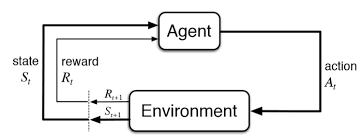
\includegraphics[scale=0.62]{rl_model.png}
\caption{Концептуальная модель обучения с подкреплением}
\label{rl_model}
\end{figure}



\section{Reinforcement learning}
\subsection{Q-learning}
Q-learning это RL-алгоритм который формирует функцию полезности $Q$ для каждого состояния, он в состоянии сравнить ожидаемую полезность доступных действий, не используя модель окружающей среды. Алгоритм считает функцию которая определяет качество состояния-действия комбинации:
\begin{equation}
Q : S \times A \rightarrow \mathbb{R}
\end{equation}
В начале таблица инициализирована одинаковыми значениями. Затем каждый момент $t$ агент выбирает действие $a_t$, получает награду $r_t$, входит в состояние $s_{t+1}$ и обновляет $Q$ используя взвешенное среднее старого значения и новой информации:

\begin{equation}
Q^{new}(s_t,a_t) \leftarrow Q(s_t,a_t)+ \alpha \cdot (r_t + \gamma \cdot \underset{a}{maxQ}(s_{t+1},a)-Q(s_t,a_t))
\end{equation}
Где $r_t$ это награда полученная за переход от состояния $s_t$ к $s_{t+1}$, $\alpha$ это скорость обучения (learning rate) $0<\alpha \leq 1$, $\gamma$ это коэффициент дисконтирования (discount factor), $Q(s_t,a_t)$ это старое значение.

\subsection{Deep Q-learning}
С ростом количества возможных состояний и действий подход, основанный на табличном представлении Q-функции быстро становится непрактичным или невозможным. Поэтому один из современных подходов заключается в использовании нейронных сетей для аппроксимации Q-функции. В рамках этого подхода нейронная сеть используется в режиме регрессии, аппроксимируя значение $Q$ для каждого возможного действия; входом сети является вектор состояния, как изображено на Рис. \ref{deep_q_learning}

\begin{figure}[h]
\centering
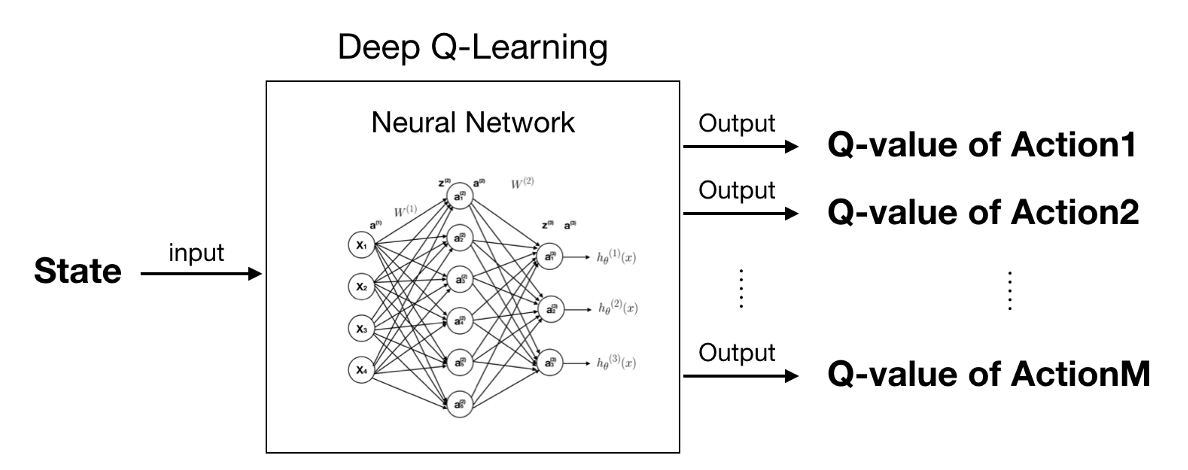
\includegraphics[scale=0.32]{deep_q_learning.png}
\caption{Deep Q-learning}
\label{deep_q_learning}
\end{figure}

Тем не менее, "прямолинейное" использование нейронной сети для представления Q-функции сопряжено с проблемами стабильности и сходимости. Основная проблема вызвана тем, что последовательные наблюдения в модели обучения с подкреплением сильно коррелированы. Чтобы обойти эту проблему группа авторов \cite{Mnih} использовала технику experience replay, в рамках которой для обучения нейронной сети на каждой итерации вместо последних значений состояний и действий использовалась небольшая случайная выборка (minibatch) из ранее наблюдавшихся состояний и действий. Такой подход приводит к декорреляции обучающей выборки и, как следствие, стабильности обучения. Еще одна модификация, которую использовала группа авторов \cite{Mnih} заключается в том, что в в процессе обучения использовалось две нейронные сети: основная, которая обучалась на каждом шаге ($Q$) и вспомогательная ($\hat{Q}$), веса которой копировались из $Q$ каждые $C$ итераций. Такой подход также заметно снижает вероятность осцилляций и расхождения при обучении. 


\section{Сжатие данных}
Программа получает на вход изображение см. рис. \ref{observation}, для начала оно обрезается только до ринга см. рис. \ref{observation_reshaped}, затем картинка заменяется на массив из трех чисел потому что различается всего 3 цвета, первый игрок, второй игрок и фон. Эти трансформации не теряют информацию. Однако даже при такой трансформации размерность вектора состояния $s_t$ остается слишком высокой поэтому для базового алгоритма Q-learning было также использовано сжатие изображения с помощью удаления каждого второго пикселя по горизонтали и по вертикали см. рис. \ref{observation_downscaled}, данное преобразование теряет информацию. Однако дает полную информацию о всех происходящих событиях, хоть и неточную. Для дальнейшего серьезного уменьшения объема информации были выделены только центры игроков (рис. \ref{observation_final}). Это достигалось с помощью взятия всех пикселей игрока, берется середина между самым высоким и низким пикселями, а затем берется середина между самым левым и правым пикселями в этой строке. Такое представление состояния теряет информацию о движениях однако имеет значительно меньшую размерность. Для снижения сложности уменьшение размерности картинки выполнялось не напрямую, а посредством деления всех значений позиций на 2.  

Для алгоритма Deep Q-learning в соответствии с \cite{Mnih} кадры сжимались до разрешения 84$\times$84, переводились в градации серого и 4 последних кадра использовались как состояние $s_t$.

\begin{figure}[H]
\begin{center}
\begin{minipage}[h]{0.4\linewidth}
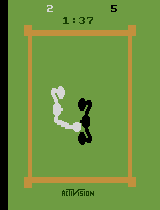
\includegraphics[width=1\linewidth]{observation.png}
\caption{Входное изображение} 
\label{observation}
\end{minipage}
\hfill
\begin{minipage}[h]{0.4\linewidth}

\includegraphics[width=1\linewidth]{observation_reshaped.png}
\caption{Обрезанное изображение}
\label{observation_reshaped}
\end{minipage}
\end{center}
\end{figure}

\begin{figure}[H]
\begin{center}
\begin{minipage}[h]{0.4\linewidth}

\includegraphics[width=1\linewidth]{observation_downscaled.png}
\caption{Сжатое изображение} 
\label{observation_downscaled}
\end{minipage}
\hfill
\begin{minipage}[h]{0.4\linewidth}
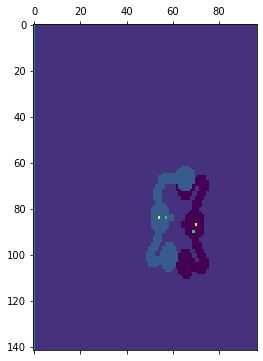
\includegraphics[width=1\linewidth]{observation_final.jpg}
\caption{Изображение с центрами}
\label{observation_final}
\end{minipage}
\end{center}
\end{figure}

\section{Результаты}

\subsection{Известные результаты других работ}

В предыдущих работах было задокументировано несколько результатов, полученных ранее другими авторами для игры Atari Boxing в стандартном окружении Arcade Learning Environment. Средние значения результатов (т.е. очков за эпизод игры) для некоторых алгоритмов приведены ниже:

\begin{center}
    \begin{tabular}{| l | l | p{7cm} |}
    \hline
    \textbf{\textit{Алгоритм}} & \textbf{\textit{Результат}} & \textbf{\textit{Описание}} \\ \hline
    Случайный агент & 0-0.1 & наши тесты, а так же \cite{Mnih}, \cite{Fortunato}  \\ \hline
    Игрок (человек) & 4.3-12 & профессиональный игровой тестировщик \cite{Mnih}, \cite{Fortunato}  \\ \hline
    SARSA-LSH & 10 & см. детали в \cite{Bellemare}\\ \hline
    SARSA-BASS & 16 & см. детали в \cite{Bellemare} \\ \hline
    DQN (Deepmind) & 71.8 & см. детали \cite{Mnih} \\ \hline
    NoisyNet-DQN & 100 & см. детали \cite{Fortunato}  \\ \hline
    *Q-learning & 17.2 & эта работа (см. далее) \\ \hline
    *Deep Q-learning & >19 & эта работа (см. далее) \\ \hline
    % Добавить результаты !!!!
    \end{tabular}
\end{center}


\subsection{Результат Q-learning}
Алгоритм Q-learning\footnote{Параметры скрипта на Python и ссылка на файл представлены в Приложении} получал на вход информацию о состоянии в виде квантованного вектора расстояния между игроками (25$\times$31) и примерного положения первого игрока в границах 9 секторов см. рис. \ref{observation_zones}, так как требовалось сжатие размерности состояний и при положении игроков не у стен поведение отличается незначительно, однако стены меняют его сильно. Таким образом программа различала 6975 состояний и была реализована с использованием табличного представления Q-функции (таблица на 6975$\times$18=125550 записей). Реализация табличного Q-learning на Python не требует использования дополнительных библиотек за исключением gym и стандартного пакета numpy. На один цикл обучения, т.е. на один эпизод игры, который длится в реальном времени 2 минуты, уходило примерно 7 секунд, причем основная часть процессорного времени тратилась на эмуляцию игрового окружения\footnote{Обучение производилось на ноутбуке Macbook Air M1}. По итогу 2500 циклов обучения программа достигла стабильной средней награды около 17 очков (рис. \ref{q-learning_graph}). Таким образом, на весь процесс обучения ушло не более 5 часов. На графике видно, что результат немного флюктуирует примерно до 13000ого цикла обучения. Это связанно исключительно с тем, что после 13000ого цикла была зафиксирована таблица и выключен эксплоринг.


\begin{figure}[H]
\begin{center}
\begin{minipage}[h]{0.3\linewidth}
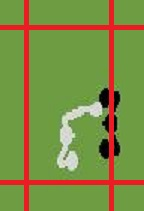
\includegraphics[width=1\linewidth]{observation_zones.jpg}
\caption{секции зоны}
\label{observation_zones}
\end{minipage}
\hfill
\begin{minipage}[h]{0.6\linewidth}
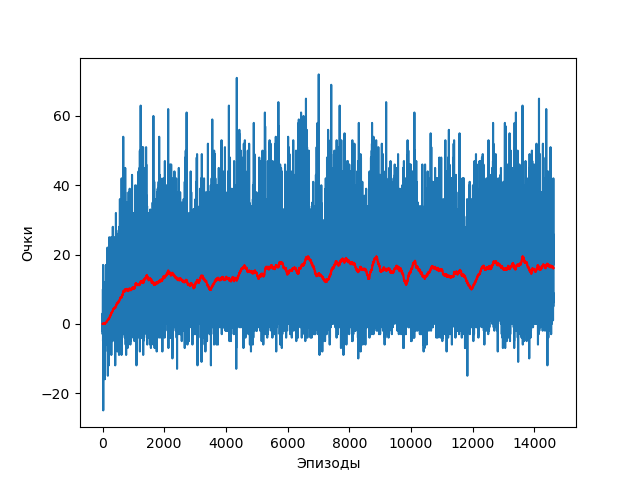
\includegraphics[width=1\linewidth]{q_learning_graph.png}
\caption{результаты Q-learning}
\label{q-learning_graph}
\end{minipage}
\end{center}
\end{figure}

\subsection{Результат Deep Q-learning}
Практическая реализация Deep Q-learning алгоритма - нетривиальная задача. Для достижения хороших результатов, как правило, требуется тонкая настройка параметров и подбор архитектуры нейронной сети, при этом обучение происходит достаточно медленно. Учитывая ограниченность вычислительных ресурсов (неигровой ноутбук) для реализации было решено остановиться на использовании библиотеки keras-rl \cite{keras-rl}. 

На вход нейронной сети подается сжатый видео-кадр игрового поля размерностью 84$\times$84 в градациях серого. Топология сети состоит из четырех скрытых слоев и одного выходного слоя, включая:
\begin{itemize}
\item сверточный слой, состоящий из 32 фильтров 8×8 с шагом 4 и функцией активации ReLU
\item сверточный слой, состоящий из 64 фильтров 4×4 с шагом 2 и функцией активации ReLU
\item сверточный слой, состоящий из 64 фильтров 3×3 с шагом 1 и функцией активации ReLU
\item полносвязный слой, состоящий из 512 элементов с функцией активации ReLU
\item выходной полносвязный слой с одним выходом для каждого действия (18)
\end{itemize}
Как можно заметить, эта архитектура и все остальные настройки\footnote{Параметры скрипта на Python и ссылка на файл представлены в Приложении} соответствуют параметрам, приведенным в \cite{Mnih}. Результаты работы нашей реализации алгоритма Deep Q-learning для первых 750 эпизодов показаны на рис. \ref{deep_q_learning_graph}. 

\begin{figure}[h]
\centering
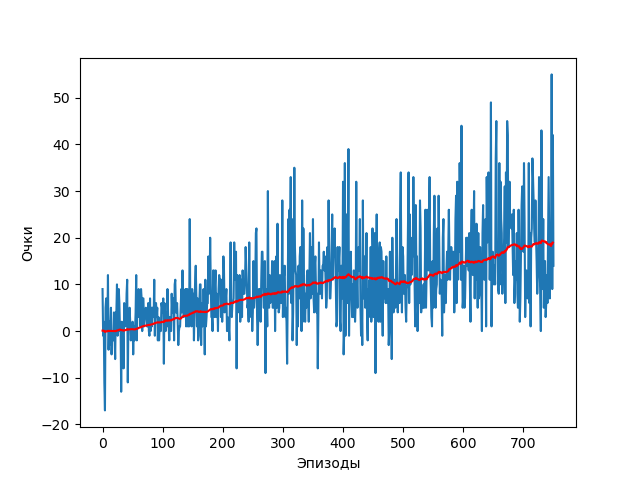
\includegraphics[scale=0.6]{deep_q_learning_graph.png}
\caption{Результаты обучения алгоритма Deep Q-learning}
\label{deep_q_learning_graph}
\end{figure}

Несмотря на то, что реализованный в работе алгоритм Deep Q-learning показал неплохой результат обучения (как минимум, лучше, чем профессиональный "живой" игрок), добиться результата приведенного в \cite{Mnih} (более 70 очков) не удалось. Дело в том, что результаты, приведенные в \cite{Mnih} получены путем обучения модели по 50 млн. кадров, то есть более 20000 эпизодов для игры Boxing. В тоже время, в нашей реализации на обработку одного эпизода уходило примерно 96 секунд, поэтому для аналогичного качества обучения нам понадобилось бы более 23 суток, а результат показанный на рис. \ref{deep_q_learning_graph} был получен после 18 часов обучения.


\section{Вывод}
По результатам исследования, табличный алгоритм Q-learning с предобработкой входных кадров специально для игры Boxing смог достичь стабильно положительных результатов за достаточно короткое время. Алгоритм Deep Q-learning может достичь более высокого результата, но при этом значительно более чувствителен к настройке параметров и выбору топологии сети, а также требует большего времени на обучение. Тем не менее, при наличии достаточных вычислительных ресурсов Deep Q-learning позволяет добиться лучшего результата не требуя специальной предобработки входных данных.

\newpage
\phantomsection
\section*{Приложение}
\addcontentsline{toc}{section}{Приложение}
\phantomsection
\subsection*{Q-learning}
\addcontentsline{toc}{subsection}{Q-learning}
Код программы приложен в файле \href{run:./Qlearning.py}{Qlearning.py}.
\begin{minted}{python}
# Параметры обучения
epsilon_decay = 0.999999
epsilon_min = 0.07
discount_factor = 0.9
learning_rate = 0.05
\end{minted}

\phantomsection
\subsection*{Deep Q-learning}
\addcontentsline{toc}{subsection}{Deep Q-learning}
Код программы приложен в файле \href{run:./DeepQlearning.py}{DeepQlearning.py}.
\begin{minted}{python}
# Параметры обучения
epsilon_max = 1
epsilon_min = 0.1
final_epsilon_frame = 1000000
discount_factor = 0.99
learning_rate = 0.00025
update_frequency = 4
minibatch_size = 32
target_network_update_frequency = 10000
replay_start_size = 50000
\end{minted}

\newpage

\phantomsection
\begin{thebibliography}{}
\addcontentsline{toc}{section}{Список используемой литературы}
    \bibitem{wikipedia} \url{https://en.wikipedia.org/wiki/Reinforcement_learning}
    \bibitem{Mnih} Mnih, V., Kavukcuoglu, K., Silver, D. et al. Human-level control through deep reinforcement learning. Nature 518, 529–533 (2015).
    \bibitem{Bellemare} Bellemare, M. G., Naddaf, Y., Veness, J. \& Bowling, M. The arcade learning environment: An evaluation platform for general agents. J. Artif. Intell. Res. 47, 253–279 (2013).
    \bibitem{Fortunato} Fortunato, M., Azar, M., Piot, B. et al. Noisy Networks for Exploration. In 6th International Conference on Learning Representations, ICLR 2018, Vancouver, BC, Canada, April 30 - May 3 (2018)
    \bibitem{keras-rl} \url{https://github.com/keras-rl/keras-rl}
\end{thebibliography}

\end{document}
